\chapter{Java Standard Library Data Structures}

The purpose of this chapter is to provide an overview on how the most basic and useful data structures work. The implementations of most higher-level languages already coded these for us, but it is important to know how each data structure works rather than blindly use the standard library.

More technical explanations of all of these can be found, mostly under the package \texttt{java.util}, in the \href{https://docs.oracle.com/javase/8/docs/api/}{Java API}.

I strongly believe that Java is better than C++ for beginning programmers. It forces people into good coding habits, and though the lack of pointers initially frustrated me, it really does make learning general concepts liked LinkedLists much easier, as the intricacies of the C++ pointer no longer distract from the larger idea.

\section{Generics}

You may or may not have seen these used before:
\begin{verbatim}
ArrayList<Integer> al = new ArrayList<Integer>();
\end{verbatim}
This means that \texttt{al} is an ArrayList of Integers. We can only add Integers into the ArrayList, and anything removed from the ArrayList is guaranteed to be an Integer. I don't think the beginning programmer needs to know how to necessarily code a class that supports generics. However, you are going to use the standard library, so you should know how to use a class that does support generics. I think standard classes are relatively straightforward to use but can be annoying to actually implement.

\textit{For simplicity, all data structures in this chapter will store Strings.}

\section{List}

A List is a collection of objects with an ordering. Users of a list have control over where in the list each object is and can access a specific element by its index, like in an array.

\subsection{ArrayList}

What is nice about an array? We can access or change any element we want in the array in $O(1)$ time. The problem is that an array has fixed length. It's not easy to append an element to the end of an array.

The fix to this is pretty simple. Why not just make a bigger array, and copy everything over to the new array? Then there's more room at the end to add a new element. This is the idea behind an ArrayList. If the backbone array runs out of space, we create a new array with double the size and keep going as if nothing happened.

\begin{center}
{
\begin{tikzpicture}[
  thick,
  myrect/.style={
    draw,
    fill=myseagreen,
    rectangle split,
    rectangle split horizontal,
    rectangle split parts=#1,
    rectangle split part align=left,
    text width=5ex,
    text centered
    },
  mycallout/.style={
    shape=rectangle callout,
    rounded corners,
    fill=mysalmon,
    callout absolute pointer={#1},
    callout pointer width=1cm
  }  
]

\node[myrect=3]
  (array1)
  {
  					\strut \texttt{"a"}
  \nodepart{two}	\strut \texttt{"b"}
  \nodepart{three}	\strut \texttt{null}
  };
\foreach \Valor [count=\Valori from 0] in {one ,two ,three }
  \node[below] at (array1.\Valor south) {\Valori};

\node[myrect=3]
  (array2)[below=of array1]
  {
  					\strut \texttt{"a"}
  \nodepart{two}	\strut \texttt{"b"}
  \nodepart{three}	\strut \texttt{"c"}
  };
\foreach \Valor [count=\Valori from 0] in {one ,two ,three }
  \node[below] at (array2.\Valor south) {\Valori};

\node[myrect=6]
  (array3)[below=of array2]
  {
  					\strut \texttt{"a"}
  \nodepart{two}	\strut \texttt{"b"}
  \nodepart{three}	\strut \texttt{"c"}
  \nodepart{four}	\strut \texttt{null}
  \nodepart{five}	\strut \texttt{null}
  \nodepart{six}	\strut \texttt{null}
  };
\foreach \Valor [count=\Valori from 0] in {one ,two ,three , four , five , six }
  \node[below] at (array3.\Valor south) {\Valori};

\node[myrect=6]
  (array4)[below=of array3]
  {
  					\strut \texttt{"a"}
  \nodepart{two}	\strut \texttt{"b"}
  \nodepart{three}	\strut \texttt{"c"}
  \nodepart{four}	\strut \texttt{"d"}
  \nodepart{five}	\strut \texttt{null}
  \nodepart{six}	\strut \texttt{null}
  };
\foreach \Valor [count=\Valori from 0] in {one ,two ,three , four , five , six }
  \node[below] at (array4.\Valor south) {\Valori};

\end{tikzpicture}
}
\end{center}

We see that there is still room in the array to add \texttt{"c"}, but to add more elements to the list, we must use a new array with double the length.

It's important to note that any given insertion to the ArrayList is either $O(n)$ or $O(1)$, but there is only one $O(n)$ insertion for every $O(n)$ $O(1)$ insertions, so we still average out to constant time.

\begin{itemize}

\item
\texttt{boolean add(String s)} -- add an element to the end of the list. (By convention, this returns \texttt{true} if the addition was successful, and \texttt{false} otherwise.)
\item
\texttt{void add(int i, String s)} -- shift everything from position \texttt{i} onward down by one, and add \texttt{s} at position \texttt{i}.
\item
\texttt{boolean contains(Object o)} -- return \texttt{true} if \texttt{o} is stored in the ArrayList, and \texttt{false} otherwise. Remember to cast \texttt{o} to a String.
\item
\texttt{String get(int i)} -- return the element stored at index \texttt{i}.
\item
\texttt{boolean isEmpty()} -- return \texttt{true} if \texttt{size() == 0}.
\item
\texttt{String remove(int i)} -- remove and return the element at index $i$ from the list. (Why is this annoying?)
\item
\texttt{String set(int i, String s)} -- replace the element stored at index \texttt{i} with \texttt{s}, and return the element that was originally at position \texttt{i}.
\item
\texttt{int size()} -- note that this is not just the length of the backbone array.
\end{itemize}

The \texttt{get} and \texttt{set} functions are very nice. They are easy to code and run in constant time. These are the bread and butter of any array. Adding at the end of the ArrayList is nice as well. \texttt{contains} is a pain, as it is $O(n)$, and adding to and removing from early in the list are more annoying.

If this is your first time seeing an ArrayList, I would suggest coding up your own. It should be relatively straightforward.

\subsection{LinkedList}

Arrays are nice for accessing, say, the seventh element in the list. We extend this to an ArrayList to implement adding and removing elements to and from the end of the list nicely. Removing elements from the beginning of the list, however, is cumbersome.

The LinkedList attempts to remedy this. It trades $O(1)$ access to any element in the list for an easier way to remove elements from either end of the list easily. Consider a chain of paper clips:

\begin{center}

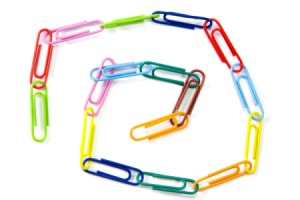
\includegraphics{images/paper_clip_chain.jpg}\footnote{\url{http://img.thrfun.com/img/078/156/paper_clip_chain_s1.jpg}}

\end{center}

It's easy to add or remove more paper clips from either end of the chain, and from any given paper clip, it's easy to access the paper clip directly previous or next to it in the chain. If we needed the seventh paper clip in the chain, we'd need to manually count, an $O(n)$ operation. However, if we then needed to remove that paper clip from the chain, it wouldn't be that hard, assuming we kept a finger on the seventh paper clip.

The standard library implements a cyclical doubly-linked list, with a dummy head. It looks something like this:

\begin{center}


\begin{tikzpicture}[
        list/.style={
            very thick, rectangle split, 
            rectangle split parts=3, draw, 
            rectangle split horizontal, minimum size=18pt,
            inner sep=5pt, text=black,
            rectangle split part fill=myseagreen
        }, 
        ->, start chain, very thick
      ]

  \node[list,on chain] (dummy) {\nodepart{second} \texttt{null}};
  \node[list,on chain] (A) {\nodepart{second} \texttt{"a"}};
  \node[list,on chain] (B) {\nodepart{second} \texttt{"b"}};
  \node[list,on chain] (C) {\nodepart{second} \texttt{"c"}};

    \path[*->] let \p1 = (dummy.three), \p2 = (dummy.center) in (\x1,\y2) edge [bend left] ($(A.one)+(0,0.2)$);
  \path[*->] let \p1 = (A.three), \p2 = (A.center) in (\x1,\y2) edge [bend left] ($(B.one)+(0,0.2)$);
  \path[*->] let \p1 = (B.three), \p2 = (B.center) in (\x1,\y2) edge [bend left] ($(C.one)+(0,0.2)$);
  
%  \draw[*->] let \p1 = (C.three), \p2 = (C.center) in (\x1,\y2) -- (dummy);

%  \draw[*->] ($(A.one)+(0.2,0.1)$) -- (dummy);
  \path[*->] ($(B.one)+(0.1,0.1)$) edge [bend left] ($(A.three)+(0,-0.05)$);
  \path[*->] ($(C.one)+(0.1,0.1)$) edge [bend left] ($(B.three)+(0,-0.05)$);
    \path[*->] ($(A.one)+(0.1,0.1)$) edge [bend left] ($(dummy.three)+(0,-0.05)$);
    
    \draw[*->] ($(C.three)+(0.0,0.2)$) -- ($(C.three)+(1.0,0.2)$) -- ($(C.three)+(1.0,-0.8)$) -- ($(dummy.one)+(-0.9,-0.8)$) -- ($(dummy.one)+(-0.9,0.2)$) -- ($(dummy.one)+(0.1,0.2)$);

    \draw[<-*] ($(C.three)+(0.0,0.0)$) -- ($(C.three)+(0.8,0.0)$) -- ($(C.three)+(0.8,-0.6)$) -- ($(dummy.one)+(-0.7,-0.6)$) -- ($(dummy.one)+(-0.7,0.0)$) -- ($(dummy.one)+(0.1,0.0)$);

\end{tikzpicture}

\end{center}

We see that each node maintains a pointer to its next neighbor and its previous neighbor, in addition to containing the String it stores. We can store this data in a class like the following:

\begin{mylstlisting}
class ListNode {
	ListNode prev, next;
    String s;
}
\end{mylstlisting}

If we were to insert an element after a ListNode \texttt{a}, it is necessary to update all pointers:

\begin{mylstlisting}
ListNode b = new ListNode();
b.prev = a;
b.next = a.next;
b.next.prev = b;
a.next = b;
\end{mylstlisting}

Since the LinkedList is symmetric, inserting an element before a node is also easy. To add something to the end of the list, simply add it before the dummy head. From here it should not be too hard to implement all the important functions of a LinkedList.

\begin{itemize}

\item \texttt{boolean add(String s)} -- add to the end.
\item \texttt{void add(int i, String s)} -- this is linear. Don't forget about 0-indexing.
\item \texttt{void addFirst()}
\item \texttt{boolean contains(Object o)}
\item \texttt{String get(int i)}
\item \texttt{String getFirst()}
\item \texttt{String getLast()}
\item \texttt{boolean isEmpty()}
\item \texttt{String remove()} -- remove the last element.
\item \texttt{String remove(int i)}
\item \texttt{String removeFirst()}
\item \texttt{String set(int i, String s)}
\item \texttt{int size()}

\end{itemize}

With a LinkedList implemented, two other data structures immediately follow.

\subsection{Stack}

A stack is is literally a stack. If we have a stack of papers, we can \textit{push} things on the top and \textit{pop} things off the top. Sometimes we \textit{peek} at what's on the top but don't actually remove anything. We never do anything with what's on the bottom. This is called \textit{LIFO}: Last In, First Out.

\begin{itemize}

\item \texttt{String push(String s)} -- pushes the item on the top of the stack, and returns the same element.

\item \texttt{String pop()} -- removes the item at the top of the stack and returns it.

\item \texttt{String peek()} -- returns the top element but does not remove it.

\end{itemize}

Java implements a Stack using an ArrayList-like structure. This works just as well, and is faster in practice, but I prefer the LinkedList structure as a mathematical concept as it is more elegant and more easily customizable.

\subsection{Queue}

A queue is like a lunch line. We \textit{add} things to the end and \textit{poll} things from the front. Sometimes we \textit{peek} at the front but don't actually remove anything. The first person in line gets served first. This is called \textit{FIFO}: First In, First Out.

\begin{itemize}

\item \texttt{boolean add(String s)}

\item \texttt{String poll()} -- removes the item at the front of the queue and returns it. Same thing as \texttt{remove()}.

\item \texttt{String peek()}

\end{itemize}

In Java, \texttt{Queue} is an interface. This means that we cannot instantiate a \texttt{Queue}, so the following statement is illegal.

\begin{mylstlisting}
Queue<String> q = new Queue<String>();
\end{mylstlisting}

Instead, we must do something like this:

\begin{mylstlisting}
Queue<String> q = new Queue<LinkedList>();
\end{mylstlisting}

This is legal because LinkedList implements Queue. Queue, however, does not extend List, so it is somewhat untruthful to place Queue under List in this book. However, I do want to stress that the LinkedList is the standard FIFO queue.

\section{PriorityQueue}

Quite often a FIFO queue is not always desirable. Maybe the String I want to remove at every given point is the one that is lexicographically least. a PriorityQueue is a Queue that allows us to do this using what is known as a \textit{heap}.

A min heap is a tree such that every node is smaller than or equal to all of its children. Pictured is a complete binary min heap, which will be of most use to us.

\begin{center}
\begin{tikzpicture}[very thick,level/.style={sibling distance=70mm/#1}]
\node [vertex] (r){\texttt{"a"}}
  child {
    node [vertex] (a) {\texttt{"b"}}
    child {
      node [vertex] {\texttt{"c"}}
      child {
        node [vertex] {\texttt{"e"}}
        child {node [vertex] {\texttt{"f"}}}
      } 
      child {
        node [vertex] {\texttt{"m"}}
      }
    }
    child {
      node [vertex] {\texttt{"n"}}
      child {node [vertex] {\texttt{"p"}}}
      child {node [vertex] {\texttt{"o"}}}
    }
  }
  child {
    node [vertex] {\texttt{"d"}}
    child {
      node [vertex] {\texttt{"g"}}
      child {node [vertex] {\texttt{"i"}}}
      child {node [vertex] {\texttt{"l"}}}
    }
    child {
      node [vertex] {\texttt{"h"}}
      child {node [vertex] {\texttt{"k"}}}
      child {node [vertex] {\texttt{"j"}}}
    }
  };
\end{tikzpicture}
\end{center}

We see that the root of the tree will always be the top element. It is tempting to use a container class with a pointer to its left and its right child. However, we have a much nicer way to store \textit{complete} binary trees with an array. Consider the following numbering of the nodes:

\begin{center}
\begin{tikzpicture}[very thick,level 1/.style={sibling distance=80mm}, level 2/.style={sibling distance=40mm}, level 3/.style={sibling distance=20mm}]
\node [splitvertex] (r){1\nodepart{lower}\texttt{"a"}}
  child {
    node [splitvertex] (a) {2\nodepart{lower}\texttt{"b"}}
    child {
      node [splitvertex] {4\nodepart{lower}\texttt{"c"}}
      child {
        node [splitvertex] {8\nodepart{lower}\texttt{"e"}}
        child {node [splitvertex] {16\nodepart{lower}\texttt{"f"}}}
      } 
      child {
        node [splitvertex] {9\nodepart{lower}\texttt{"m"}}
      }
    }
    child {
      node [splitvertex] {5\nodepart{lower}\texttt{"n"}}
      child {node [splitvertex] {10\nodepart{lower}\texttt{"p"}}}
      child {node [splitvertex] {11\nodepart{lower}\texttt{"o"}}}
    }
  }
  child {
    node [splitvertex] {3\nodepart{lower}\texttt{"d"}}
    child {
      node [splitvertex] {6\nodepart{lower}\texttt{"g"}}
      child {node [splitvertex] {12\nodepart{lower}\texttt{"i"}}}
      child {node [splitvertex] {13\nodepart{lower}\texttt{"l"}}}
    }
    child {
      node [splitvertex] {7\nodepart{lower}\texttt{"h"}}
      child {node [splitvertex] {14\nodepart{lower}\texttt{"k"}}}
      child {node [splitvertex] {15\nodepart{lower}\texttt{"j"}}}
    }
  };
\end{tikzpicture}
\end{center}

We see that every number from 1 to 16 is used, and for every node, if the index associated with it is $i$, the left child is $2i$, and the right child is $2i+1$. This leads to a very natural implementation of the tree in an array:

\begin{center}
{
\begin{tikzpicture}[
  thick,
  myrect/.style={
    draw,
    fill=myseagreen,
    rectangle split,
    rectangle split horizontal,
    rectangle split parts=#1,
    rectangle split part align=left,
    text centered
    },
  mycallout/.style={
    shape=rectangle callout,
    rounded corners,
    fill=mysalmon,
    callout absolute pointer={#1},
    callout pointer width=1cm
  }  
]

\node[myrect=17]
  (array)
  {
  					\strut \texttt{null}
  \nodepart{two}	\strut \texttt{"a"}
  \nodepart{three}	\strut \texttt{"b"}
  \nodepart{four}	\strut \texttt{"d"}
  \nodepart{five}	\strut \texttt{"c"}
  \nodepart{six}	\strut \texttt{"n"}
  \nodepart{seven}	\strut \texttt{"g"}
  \nodepart{eight}	\strut \texttt{"h"}
  \nodepart{nine}	\strut \texttt{"e"}
  \nodepart{ten}	\strut \texttt{"m"}
  \nodepart{eleven}	\strut \texttt{"p"}
  \nodepart{twelve}	\strut \texttt{"o"}
  \nodepart{thirteen}	\strut \texttt{"i"}
  \nodepart{fourteen}	\strut \texttt{"l"}
  \nodepart{fifteen}	\strut \texttt{"k"}
  \nodepart{sixteen}	\strut \texttt{"j"}
  \nodepart{seventeen}	\strut \texttt{"f"}
  };
\foreach \Valor [count=\Valori from 0] in {one ,two ,three ,four ,five ,six ,seven ,eight ,nine ,ten ,eleven ,twelve ,thirteen ,fourteen ,fifteen ,sixteen ,seventeen }
  \node[below] at (array.\Valor south) {\Valori};

\end{tikzpicture}
}
\end{center}

How do we add elements to our heap, while maintaining the heap qualities? Well, let's just add it to the very end and see what we get. Suppose we are to add \texttt{"b"} to the tree.

\begin{center}
\begin{tikzpicture}[very thick,level 1/.style={sibling distance=80mm}, level 2/.style={sibling distance=40mm}, level 3/.style={sibling distance=20mm}]
\node [splitvertex] (r){1\nodepart{lower}\texttt{"a"}}
  child {
    node [splitvertex] (a) {2\nodepart{lower}\texttt{"b"}}
    child {
      node [splitvertex] {4\nodepart{lower}\texttt{"c"}}
      child {
        node [splitvertex] {8\nodepart{lower}\texttt{"e"}}
        child {node [splitvertex] {16\nodepart{lower}\texttt{"f"}}}
        child {node [splitvertex, fill=mysalmon] {17\nodepart{lower}\texttt{"b"}}}
      } 
      child {
        node [splitvertex] {9\nodepart{lower}\texttt{"m"}}
      }
    }
    child {
      node [splitvertex] {5\nodepart{lower}\texttt{"n"}}
      child {node [splitvertex] {10\nodepart{lower}\texttt{"p"}}}
      child {node [splitvertex] {11\nodepart{lower}\texttt{"o"}}}
    }
  }
  child {
    node [splitvertex] {3\nodepart{lower}\texttt{"d"}}
    child {
      node [splitvertex] {6\nodepart{lower}\texttt{"g"}}
      child {node [splitvertex] {12\nodepart{lower}\texttt{"i"}}}
      child {node [splitvertex] {13\nodepart{lower}\texttt{"l"}}}
    }
    child {
      node [splitvertex] {7\nodepart{lower}\texttt{"h"}}
      child {node [splitvertex] {14\nodepart{lower}\texttt{"k"}}}
      child {node [splitvertex] {15\nodepart{lower}\texttt{"j"}}}
    }
  };
\end{tikzpicture}
\end{center}

Well, \texttt{"b"} comes before \texttt{"e"} in the alphabet, so let's swap the nodes. We are guaranteed that \texttt{"b"} should come before the other child (in this case, \texttt{"f"}) by the transitive property.

\begin{center}
\begin{tikzpicture}[very thick,level 1/.style={sibling distance=80mm}, level 2/.style={sibling distance=40mm}, level 3/.style={sibling distance=20mm}]
\node [splitvertex] (r){1\nodepart{lower}\texttt{"a"}}
  child {
    node [splitvertex] (a) {2\nodepart{lower}\texttt{"b"}}
    child {
      node [splitvertex] {4\nodepart{lower}\texttt{"c"}}
      child {
        node [splitvertex, fill=mysalmon] {8\nodepart{lower}\texttt{"b"}}
        child {node [splitvertex] {16\nodepart{lower}\texttt{"f"}}}
        child {node [splitvertex, fill=mysalmon] {17\nodepart{lower}\texttt{"e"}}}
      } 
      child {
        node [splitvertex] {9\nodepart{lower}\texttt{"m"}}
      }
    }
    child {
      node [splitvertex] {5\nodepart{lower}\texttt{"n"}}
      child {node [splitvertex] {10\nodepart{lower}\texttt{"p"}}}
      child {node [splitvertex] {11\nodepart{lower}\texttt{"o"}}}
    }
  }
  child {
    node [splitvertex] {3\nodepart{lower}\texttt{"d"}}
    child {
      node [splitvertex] {6\nodepart{lower}\texttt{"g"}}
      child {node [splitvertex] {12\nodepart{lower}\texttt{"i"}}}
      child {node [splitvertex] {13\nodepart{lower}\texttt{"l"}}}
    }
    child {
      node [splitvertex] {7\nodepart{lower}\texttt{"h"}}
      child {node [splitvertex] {14\nodepart{lower}\texttt{"k"}}}
      child {node [splitvertex] {15\nodepart{lower}\texttt{"j"}}}
    }
  };
\end{tikzpicture}
\end{center}

One more swap...

\begin{center}
\begin{tikzpicture}[very thick,level 1/.style={sibling distance=80mm}, level 2/.style={sibling distance=40mm}, level 3/.style={sibling distance=20mm}]
\node [splitvertex] (r){1\nodepart{lower}\texttt{"a"}}
  child {
    node [splitvertex] (a) {2\nodepart{lower}\texttt{"b"}}
    child {
      node [splitvertex, fill=mysalmon] {4\nodepart{lower}\texttt{"b"}}
      child {
        node [splitvertex, fill=mysalmon] {8\nodepart{lower}\texttt{"c"}}
        child {node [splitvertex] {16\nodepart{lower}\texttt{"f"}}}
        child {node [splitvertex] {17\nodepart{lower}\texttt{"e"}}}
      } 
      child {
        node [splitvertex] {9\nodepart{lower}\texttt{"m"}}
      }
    }
    child {
      node [splitvertex] {5\nodepart{lower}\texttt{"n"}}
      child {node [splitvertex] {10\nodepart{lower}\texttt{"p"}}}
      child {node [splitvertex] {11\nodepart{lower}\texttt{"o"}}}
    }
  }
  child {
    node [splitvertex] {3\nodepart{lower}\texttt{"d"}}
    child {
      node [splitvertex] {6\nodepart{lower}\texttt{"g"}}
      child {node [splitvertex] {12\nodepart{lower}\texttt{"i"}}}
      child {node [splitvertex] {13\nodepart{lower}\texttt{"l"}}}
    }
    child {
      node [splitvertex] {7\nodepart{lower}\texttt{"h"}}
      child {node [splitvertex] {14\nodepart{lower}\texttt{"k"}}}
      child {node [splitvertex] {15\nodepart{lower}\texttt{"j"}}}
    }
  };
\end{tikzpicture}
\end{center}

And now we have the heap property restored. As the tree has depth at most $\log{n}$, this process is $O(\log{n})$.

To remove the root from the heap, we replace the root with the last leaf:

\begin{center}
\begin{tikzpicture}[very thick,level 1/.style={sibling distance=80mm}, level 2/.style={sibling distance=40mm}, level 3/.style={sibling distance=20mm}]
\node [splitvertex, fill=mysalmon] (r){1\nodepart{lower}\texttt{"e"}}
  child {
    node [splitvertex] (a) {2\nodepart{lower}\texttt{"b"}}
    child {
      node [splitvertex] {4\nodepart{lower}\texttt{"b"}}
      child {
        node [splitvertex] {8\nodepart{lower}\texttt{"c"}}
        child {node [splitvertex] {16\nodepart{lower}\texttt{"f"}}}
      } 
      child {
        node [splitvertex] {9\nodepart{lower}\texttt{"m"}}
      }
    }
    child {
      node [splitvertex] {5\nodepart{lower}\texttt{"n"}}
      child {node [splitvertex] {10\nodepart{lower}\texttt{"p"}}}
      child {node [splitvertex] {11\nodepart{lower}\texttt{"o"}}}
    }
  }
  child {
    node [splitvertex] {3\nodepart{lower}\texttt{"d"}}
    child {
      node [splitvertex] {6\nodepart{lower}\texttt{"g"}}
      child {node [splitvertex] {12\nodepart{lower}\texttt{"i"}}}
      child {node [splitvertex] {13\nodepart{lower}\texttt{"l"}}}
    }
    child {
      node [splitvertex] {7\nodepart{lower}\texttt{"h"}}
      child {node [splitvertex] {14\nodepart{lower}\texttt{"k"}}}
      child {node [splitvertex] {15\nodepart{lower}\texttt{"j"}}}
    }
  };
  \node [splitvertex, fill=mysalmon] [right=5cm of r]{17\nodepart{lower}\texttt{"a"}};
\end{tikzpicture}
\end{center}

We perform a series of swaps to restore the heap property. We always want to choose the smaller child to swap until the heap property is satisfied.

\begin{center}
\begin{tikzpicture}[very thick,level 1/.style={sibling distance=80mm}, level 2/.style={sibling distance=40mm}, level 3/.style={sibling distance=20mm}, level distance=12mm, level 4/.style={level distance=15mm}]
\node [splitvertex, fill=mysalmon] (r){1\nodepart{lower}\texttt{"b"}}
  child {
    node [splitvertex, fill=mysalmon] (a) {2\nodepart{lower}\texttt{"e"}}
    child {
      node [splitvertex] {4\nodepart{lower}\texttt{"b"}}
      child {
        node [splitvertex] {8\nodepart{lower}\texttt{"c"}}
        child {node [splitvertex] {16\nodepart{lower}\texttt{"f"}}}
      } 
      child {
        node [splitvertex] {9\nodepart{lower}\texttt{"m"}}
      }
    }
    child {
      node [splitvertex] {5\nodepart{lower}\texttt{"n"}}
      child {node [splitvertex] {10\nodepart{lower}\texttt{"p"}}}
      child {node [splitvertex] {11\nodepart{lower}\texttt{"o"}}}
    }
  }
  child {
    node [splitvertex] {3\nodepart{lower}\texttt{"d"}}
    child {
      node [splitvertex] {6\nodepart{lower}\texttt{"g"}}
      child {node [splitvertex] {12\nodepart{lower}\texttt{"i"}}}
      child {node [splitvertex] {13\nodepart{lower}\texttt{"l"}}}
    }
    child {
      node [splitvertex] {7\nodepart{lower}\texttt{"h"}}
      child {node [splitvertex] {14\nodepart{lower}\texttt{"k"}}}
      child {node [splitvertex] {15\nodepart{lower}\texttt{"j"}}}
    }
  };
  \node [splitvertex] [right=5cm of r]{17\nodepart{lower}\texttt{"a"}};
\end{tikzpicture}
\end{center}

\begin{center}
\begin{tikzpicture}[very thick,level 1/.style={sibling distance=80mm}, level 2/.style={sibling distance=40mm}, level 3/.style={sibling distance=20mm}, level distance=12mm, level 4/.style={level distance=15mm}]
\node [splitvertex] (r){1\nodepart{lower}\texttt{"b"}}
  child {
    node [splitvertex, fill=mysalmon] (a) {2\nodepart{lower}\texttt{"b"}}
    child {
      node [splitvertex, fill=mysalmon] {4\nodepart{lower}\texttt{"e"}}
      child {
        node [splitvertex] {8\nodepart{lower}\texttt{"c"}}
        child {node [splitvertex] {16\nodepart{lower}\texttt{"f"}}}
      } 
      child {
        node [splitvertex] {9\nodepart{lower}\texttt{"m"}}
      }
    }
    child {
      node [splitvertex] {5\nodepart{lower}\texttt{"n"}}
      child {node [splitvertex] {10\nodepart{lower}\texttt{"p"}}}
      child {node [splitvertex] {11\nodepart{lower}\texttt{"o"}}}
    }
  }
  child {
    node [splitvertex] {3\nodepart{lower}\texttt{"d"}}
    child {
      node [splitvertex] {6\nodepart{lower}\texttt{"g"}}
      child {node [splitvertex] {12\nodepart{lower}\texttt{"i"}}}
      child {node [splitvertex] {13\nodepart{lower}\texttt{"l"}}}
    }
    child {
      node [splitvertex] {7\nodepart{lower}\texttt{"h"}}
      child {node [splitvertex] {14\nodepart{lower}\texttt{"k"}}}
      child {node [splitvertex] {15\nodepart{lower}\texttt{"j"}}}
    }
  };
  \node [splitvertex] [right=5cm of r]{17\nodepart{lower}\texttt{"a"}};
\end{tikzpicture}
\end{center}

\begin{center}
\begin{tikzpicture}[very thick,level 1/.style={sibling distance=80mm}, level 2/.style={sibling distance=40mm}, level 3/.style={sibling distance=20mm}, level distance=12mm, level 4/.style={level distance=15mm}]
\node [splitvertex] (r){1\nodepart{lower}\texttt{"b"}}
  child {
    node [splitvertex] (a) {2\nodepart{lower}\texttt{"b"}}
    child {
      node [splitvertex, fill=mysalmon] {4\nodepart{lower}\texttt{"c"}}
      child {
        node [splitvertex, fill=mysalmon] {8\nodepart{lower}\texttt{"e"}}
        child {node [splitvertex] {16\nodepart{lower}\texttt{"f"}}}
      } 
      child {
        node [splitvertex] {9\nodepart{lower}\texttt{"m"}}
      }
    }
    child {
      node [splitvertex] {5\nodepart{lower}\texttt{"n"}}
      child {node [splitvertex] {10\nodepart{lower}\texttt{"p"}}}
      child {node [splitvertex] {11\nodepart{lower}\texttt{"o"}}}
    }
  }
  child {
    node [splitvertex] {3\nodepart{lower}\texttt{"d"}}
    child {
      node [splitvertex] {6\nodepart{lower}\texttt{"g"}}
      child {node [splitvertex] {12\nodepart{lower}\texttt{"i"}}}
      child {node [splitvertex] {13\nodepart{lower}\texttt{"l"}}}
    }
    child {
      node [splitvertex] {7\nodepart{lower}\texttt{"h"}}
      child {node [splitvertex] {14\nodepart{lower}\texttt{"k"}}}
      child {node [splitvertex] {15\nodepart{lower}\texttt{"j"}}}
    }
  };
  \node [splitvertex] [right=5cm of r]{17\nodepart{lower}\texttt{"a"}};
\end{tikzpicture}
\end{center}

And we are done. Once again, this takes at most $\log(N)$ swaps. This idea can be extended to removing or changing the value of any node we'd like from a tree -- this is particularly useful for Dijkstra later.

Remember to implement your heap in an array or ArrayList!

\begin{itemize}

\item \texttt{boolean add(String s)}

\item \texttt{boolean isEmpty()}

\item \texttt{String poll()}

\item \texttt{String peek()}

\item \texttt{int size()}

\end{itemize}

\section{Set}

A Set is a collection of objects with no duplicate elements. Set is a Java interface. Note that the data structures discussed in this section can be extended to become multisets, but Java implementations of these explicitly disallow multiplicity.

\subsection{TreeSet}

A TreeSet is Java's implementation of a \textit{binary search tree} (BST). A binary search tree is a tree where every node is greater than every node in its left subtree and less than every node in its right subtree. As with a heap, to use a BST, we need to impose some kind of ordering on the elements stored.

\begin{center}
\begin{tikzpicture}[very thick,level/.style={sibling distance=70mm/#1}]
\node [vertex] (r){\texttt{"m"}}
  child {
    node [vertex] {\texttt{"g"}}
    child {
      node [vertex] {\texttt{"c"}}
      child {
        node [vertex] {\texttt{"b"}}
        child {node [vertex] {\texttt{"a"}}}
        child[missing]
      } 
      child {
        node [vertex] {\texttt{"e"}}
      }
    }
    child {
      node [vertex] {\texttt{"j"}}
      child {node [vertex] {\texttt{"h"}}}
      child {node [vertex] {\texttt{"k"}}}
    }
  }
  child {
    node [vertex] {\texttt{"t"}}
    child {
      node [vertex] {\texttt{"r"}}
      child[missing]
      child {node [vertex] {\texttt{"s"}}}
    }
    child[missing]
  };
\end{tikzpicture}
\end{center}

The tree need not be complete. Because it is not complete, there is no way to nicely bound the size of the array we would need if we were to use the same storage method as with the heap. Thus, we are forced to use a TreeNode, with left and right pointers. This is also problematic when determining guarantees on time complexities later, but the ways to solve this problem are pretty complicated so we'll ignore them for now.

Given the name of the tree, searching for an element within the tree is quite natural, and similar to a binary search. Compare the element to be searched for with the current node. If they are equal, we are done; otherwise, search the appropriate left or right subtree. As with most structures and algorithms with a binary search structure, this operation lends itself nicely to recursion. If the tree is reasonably nice, we expect to complete this in $O(\log{n})$ time, but searching can be as bad as linear if the tree looks like a LinkedList.

Adding an element is also natural. As our tree represents a set, it will not contain the same element twice. We trace down until we hit a null pointer, and add the element in the appropriate spot. Let's add a \texttt{"p"} to the BST:

\begin{center}
\begin{tikzpicture}[very thick,level/.style={sibling distance=70mm/#1}]
\node [vertex, fill=mysalmon] (r){\texttt{"m"}}
  child {
    node [vertex] {\texttt{"g"}}
    child {
      node [vertex] {\texttt{"c"}}
      child {
        node [vertex] {\texttt{"b"}}
        child {node [vertex] {\texttt{"a"}}}
        child[missing]
      } 
      child {
        node [vertex] {\texttt{"e"}}
      }
    }
    child {
      node [vertex] {\texttt{"j"}}
      child {node [vertex] {\texttt{"h"}}}
      child {node [vertex] {\texttt{"k"}}}
    }
  }
  child {
    node [vertex, fill=mysalmon] {\texttt{"t"}}
    child {
      node [vertex, fill=mysalmon] {\texttt{"r"}}
      child {node [vertex, fill=mysalmon] {\texttt{"p"}}}
      child {node [vertex] {\texttt{"s"}}}
    }
    child[missing]
  };
\end{tikzpicture}
\end{center}

Deleting an element is the annoying part. Unfortunately, there's not much we can do besides casework.

Removing a leaf, like \texttt{"a"}, from the tree is very easy. Removing a node with only once child, like \texttt{"t"}, is also relatively straightforward.

\begin{center}
\begin{tikzpicture}[very thick,level/.style={sibling distance=70mm/#1}]
\node [vertex] (r){\texttt{"m"}}
  child {
    node [vertex] {\texttt{"g"}}
    child {
      node [vertex] {\texttt{"c"}}
      child {
        node [vertex] {\texttt{"b"}}
        child {node [vertex,fill=mysalmon] {\texttt{"a"}}}
        child[missing]
      } 
      child {
        node [vertex] {\texttt{"e"}}
      }
    }
    child {
      node [vertex] {\texttt{"j"}}
      child {node [vertex] {\texttt{"h"}}}
      child {node [vertex] {\texttt{"k"}}}
    }
  }
  child {
    node [vertex, fill=mysalmon] {\texttt{"t"}}
    child {
      node [vertex] {\texttt{"r"}}
      child {node [vertex] {\texttt{"p"}}}
      child {node [vertex] {\texttt{"s"}}}
    }
    child[missing]
  };
\end{tikzpicture}
\end{center}

Now, removing an element with two children is tricky. We'll try to remove \texttt{"g"}. Consider the least element in the right subtree of \texttt{"g"}, which in this case is \texttt{"h"}. We find \texttt{"h"} by always choosing the left child on the right subtree until we cannot go any further. This must be the least element.

\begin{center}
\begin{tikzpicture}[very thick,level/.style={sibling distance=70mm/#1}]
\node [vertex] (r){\texttt{"m"}}
  child {
    node [vertex, fill=mysalmon] {\texttt{"g"}}
    child {
      node [vertex] {\texttt{"c"}}
      child {
        node [vertex] {\texttt{"b"}}
      } 
      child {
        node [vertex] {\texttt{"e"}}
      }
    }
    child {
      node [vertex] {\texttt{"j"}}
      child {node [vertex] {\texttt{"h"}}}
      child {node [vertex] {\texttt{"k"}}}
    }
  }
  child {
      node [vertex] {\texttt{"r"}}
      child {node [vertex] {\texttt{"p"}}}
      child {node [vertex] {\texttt{"s"}}}
  };
\end{tikzpicture}
\end{center}

Note that \texttt{"h"} has either no children or only one child, and that nodes like these are easy to remove. We then change the value of the node containing \texttt{"g"} to \texttt{"h"}, which is legal since \texttt{"h"} is the least element, and remove \texttt{"h"} from the right subtree, and we are done.

\begin{center}
\begin{tikzpicture}[very thick,level/.style={sibling distance=70mm/#1}]
\node [vertex] (r){\texttt{"m"}}
  child {
    node [vertex, fill=mysalmon] {\texttt{"h"}}
    child {
      node [vertex] {\texttt{"c"}}
      child {
        node [vertex] {\texttt{"b"}}
      } 
      child {
        node [vertex] {\texttt{"e"}}
      }
    }
    child {
      node [vertex] {\texttt{"j"}}
      child {node [vertex, fill=mysalmon] {\texttt{"h"}}}
      child {node [vertex] {\texttt{"k"}}}
    }
  }
  child {
      node [vertex] {\texttt{"r"}}
      child {node [vertex] {\texttt{"p"}}}
      child {node [vertex] {\texttt{"s"}}}
  };
\end{tikzpicture}
\end{center}

\begin{center}
\begin{tikzpicture}[very thick,level/.style={sibling distance=70mm/#1}]
\node [vertex] (r){\texttt{"m"}}
  child {
    node [vertex] {\texttt{"h"}}
    child {
      node [vertex] {\texttt{"c"}}
      child {
        node [vertex] {\texttt{"b"}}
      } 
      child {
        node [vertex] {\texttt{"e"}}
      }
    }
      child {node [vertex] {\texttt{"j"}}
      	child[missing]
        child {
        	node[vertex]{\texttt{"k"}}
        }
      }
  }
  child {
      node [vertex] {\texttt{"r"}}
      child {node [vertex] {\texttt{"p"}}}
      child {node [vertex] {\texttt{"s"}}}
  };
\end{tikzpicture}
\end{center}

A standard BST has $O(\log{n})$ operations if the tree is ``nice'', but each operation can be $O(n)$ in the worst case. We need to find a way to automatically balance the BST such that we avoid linear time complexities.

A red-black tree is a self-balancing BST that guarantees $O(\log{n})$ operations by making sure the height of the tree grows logarithmically. It is implemented in Java's TreeSet, so while the BST I described above does not guarantee nice time bounds, Java's implementation does.

I don't think learning exactly how a red-black tree works is particularly useful for the beginning programmer. How exactly a red-black tree works, together with some more balanced binary search trees which are useful on the competitive scene, are covered in a later chapter.

Here are some notable functions TreeSet implements. You don't need to implement everything -- \texttt{add()}, \texttt{remove()}, and \texttt{contains()} are the most important.

\begin{itemize}

\item
\texttt{boolean add(String s)}

\item
\texttt{String ceiling(String s)} -- the least element in the set greater than or equal to \texttt{s}, or \texttt{null} if there is no such element.

\item
\texttt{boolean contains(Object o)}

\item
\texttt{String first()} -- the least element in the set.

\item
\texttt{String floor(String s)} -- the greatest element in the set less than or equal to \texttt{s}, or \texttt{null} if there is no such element.

\item
\texttt{String higher(String s)} -- the least element in the set strictly greater than \texttt{s}, or \texttt{null} if there is no such element.

\item
\texttt{boolean isEmpty()}

\item
\texttt{String last()} -- the greatest element in the set.

\item
\texttt{String lower(String s)} -- the greatest element in the set strictly less than \texttt{s}, or \texttt{null} if there is no such element.

\item
\texttt{boolean remove(Object o)}

\item
\texttt{int size()}

\end{itemize}

Since the TreeSet is ordered, iterating over a TreeSet will also be in order.

\subsection{HashSet}

A HashSet is a way for us to store objects when we do not require a natural ordering on the set. As with the TreeSet, we want to be able to check whether an element is in our set or not quickly. We do this with the help of a \textit{hash function}. Every Java Object supports the \texttt{hashCode()} function. We usually want to map an object with an integer hash, so that we can store the values in an array. For example, let us define the following hash for Strings:

\begin{mylstlisting}
public int hashCode() {
	int hash = 0;
    for(int k = 0; k < length(); k++) {
		hash *= 31;
        hash += (int) (charAt(k));
    }
    return hash;
}
\end{mylstlisting}

\texttt{a.equals(b)} should imply \texttt{a.hashCode() == b.hashCode()}. This function produces the same result as the actual \texttt{hashCode()} function in the String class. However, this is not quite what we want for our HashSet, because in the end we wish to be able to store the objects in some kind of array. This hash not only returns integers that can be very large, they can also be negative, and thus are not suitable as array indices. The natural way to fix this is to take the hash modulo the size of the array we want.

\begin{mylstlisting}
String[] table = new String[10007];
int index(String s) {
	int i = s.hashCode() % table.length;
    if(i >= 0)
    	return i;
	return i + table.length;
}
\end{mylstlisting}

We chose the number 10007 because it is a prime number, and primes are generally nice when taking a number modulo something else, as integers modulo a prime form a field. Remember that a negative number \texttt{\%} another number is not necessarily positive, so we need to be a little careful.

From here, adding an element to the HashSet and checking if an element is contained both seem straightforward:

\begin{mylstlisting}
boolean add (String s) {
	table[index(s)] = s;
    return true;
}
boolean contains(Object o) {
    int i = index((String) o);
	return table[i] != null && table[i].equals(o);
}
\end{mylstlisting}

\texttt{null} is always annoying to deal with, and will have to be handled separately.

However, one problem quickly arises. Two Strings may map to the same index in the array. We call this a \textit{collision}. The easiest way to handle a collision is by \textit{chaining}. We change the hash table to store a LinkedList instead of a single element in the event of a collision. Java once implemented this method of resolving collisions, but recently changed the LinkedList to a BST in Java 8.

\begin{itemize}

\item
\texttt{boolean add(String s)}

\item
\texttt{boolean contains(Object o)}

\item
\texttt{boolean isEmpty()}

\item
\texttt{boolean remove(Object o)}

\item
\texttt{int size()}

\end{itemize}

\section{Map}

A Map is simply an extension of a Set. It stores a mapping that takes a key to a value. Map is a Java Interface. Generics for Maps therefore have two arguments. Consider the following Map from Strings to Strings.

\begin{mylstlisting}
Map<String, String> email = new TreeMap<String, String>();
email.put("Samuel Hsiang", "samuel.c.hsiang@gmail.com");
\end{mylstlisting}

The keys of a Map form a Set, though the Values need not be unique.

The TreeMap is the Map variant of the TreeSet; similarly, the HashMap is the Map variant of the HashSet.

All useful Set functions have a Map counterpart. The following additional functions are of use.

\begin{itemize}

\item
\texttt{String get(Object k)} -- return the value assigned to \texttt{k}.

\item
\texttt{Set<String> keySet()} -- returns the set of keys.

\item
\texttt{Integer put(String k, String v)} -- assigns the value \texttt{k} to the key \texttt{v}, and returns the old value assigned to \texttt{k}.

\end{itemize}

\section{BigInteger}

BigInteger is in \texttt{java.math} for times when int and long just aren't large enough. The way BigInteger works is it stores a number as an array of ints. Each value in the array represents a digit in some very large base. Addition and subtraction can be done in the standard way. Generally multiplying two BigIntegers is not necessary on contests, but it can be sped up using Karatsuba or the FFT.

\section{C++ Analogs}

\begin{itemize}

\item \texttt{ArrayList} -- \texttt{vector}
\item \texttt{LinkedList} -- \texttt{list} or \texttt{deque}
\item \texttt{Stack} -- \texttt{stack}
\item \texttt{Queue} -- \texttt{queue}
\item \texttt{PriorityQueue} -- \texttt{priority\_queue}, but note that \texttt{priority\_queue} pops \textit{max} element first
\item \texttt{TreeSet} -- \texttt{set}
\item \texttt{HashSet} -- \texttt{unordered\_set}, C++11
\item \texttt{TreeMap} -- \texttt{map}
\item \texttt{HashMap} -- \texttt{unordered\_map}, C++11
\item \texttt{BigInteger} -- no equivalent

\end{itemize}
